
%==========================================================================

\begin{frame}[fragile]

  {\Huge Asynchronicity and Streams}

  \vspace{10pt}

	{\large The (non-)blocking behavior of Kokkos operations.}

  \vspace{20pt}

  \textbf{Learning objectives:}
  \begin{itemize}
    \item {What are blocking and non-blocking operations in Kokkos.}
    \item {What kind of work can overlap.}
    \item {How to wait for completion.}
    \item {How to run kernels simultaneously on a GPU.}
  \end{itemize}

  \vspace{-20pt}

\end{frame}

%==========================================================================

\begin{frame}[fragile]{Kokkos Operations Are Non-Blocking}
\textbf{Most operations in Kokkos are non-blocking}

\begin{itemize}
  \item{The caller returns before the operation is finished}
  \item{The caller can do other things, while operations are executing}
\end{itemize}

\pause

\textbf{So what is the ordering behavior?}

\begin{itemize}
  \item{Execution Spaces have an ordered execution queue}
  \item{The queue is first-in/first-out (FIFO)}
\end{itemize}

\pause
\begin{block}{Important Point}
  Execution Spaces execute operations in dispatch order.
\end{block}

\end{frame}

%==========================================================================

\begin{frame}[fragile]{Execution Resources in Kokkos}
\textbf{Execution Space Instances}

\begin{itemize}
  \item{Each unique \textbf{Instance} of an execution space has its own queue}
  \item{Execution Policies can take an instance as the first argument}
  \item{deep\_copy can take an instance as a first argument}
  \item{For every \textbf{Execution Space Type} there is a \textbf{default instance}}
	  \begin{itemize}
		  \item{It is a singleton}
		  \item{The \textbf{default instance} is returned by the default constructor}
		  \item{Used if no specific instance is provided}
	  \end{itemize}
\end{itemize}

\pause
\begin{code}[linebackgroundcolor={},keywords={L1,L2,policy_device}]
// This is equivalent:
RangePolicy<ExecSpace> 
  policy_1(0, N);
RangePolicy<ExecSpace> 
  policy_2(ExecSpace(), 0, N);
\end{code}


\end{frame}

%==========================================================================

\begin{frame}[fragile]{Naming Conventions for Examples}
\textbf{We use the following conventions in subsequent slides}
\begin{code}[linebackgroundcolor={},keywords={device,host,policy_d,policy_device,policy_h,policy_host,policy_d1,policy_d2,policy_h1,policy_h2}]
// Execution Space types
using device = Kokkos::DefaultExecutionSpace;
using host = Kokkos::DefaultHostExecutionSpace;

// Execution Space instances
device dev1(..), dev2(..)
host host1(..), host2(..);

// Execution Policies
RangePolicy<device> policy_d(0,N), policy_device(0,N);
RangePolicy<host> policy_h(0,N), policy_host(0,N);
RangePolicy<device> policy_d1(dev1,0,N), policy_d2(dev2,0,N);
RangePolicy<host> policy_h1(host1,0,N), policy_h2(host2,0,N);

// Functors/Lambdas for parallel_for
auto L1 = KOKKOS_LAMBDA(int i) {...};
auto L2 = ...; auto L3 = ...; auto L4 = ...; auto L5 = ...;
// Functors/Lambdas for parallel_reduce
auto R1 = KOKKOS_LAMBDA(int i, double& lsum) {...};
\end{code}
\end{frame}
%==========================================================================

\begin{frame}[fragile]{Simple Dispatch}
  \textbf{Most Kokkos Operations are Asynchronous}
  \begin{itemize}
    \item{Best to assume all of them are asynchronous}
    \item{They overlap with work in the process thread}
    \item{Use \texttt{Kokkos::fence()} to wait for completion}
  \end{itemize}

  \begin{columns}[]
    \begin{column}{.67\textwidth}

       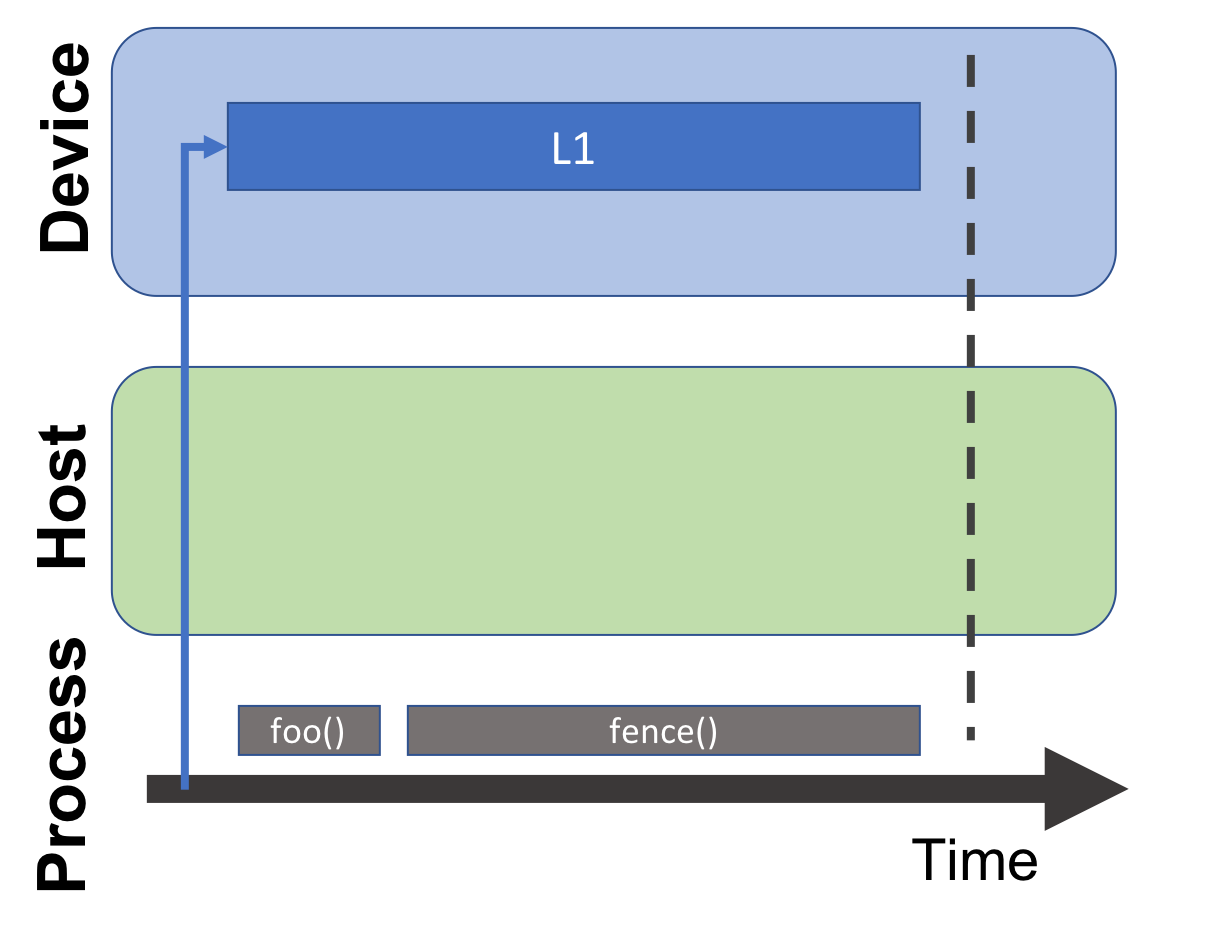
\includegraphics[width=0.95\textwidth]{figures/streams-fig0} 
 
    \end{column}

    \begin{column}{.33\textwidth}
	    \begin{code}[linebackgroundcolor={},keywords={L1,L2,policy_device}]
RangePolicy<> 
  policy_device(0,N)
FunctorL1 L1(...);

parallel_for("L1", 
  policy_device, L1);
foo();
fence();
      \end{code}
    \end{column}
  \end{columns}
\end{frame}
%==========================================================================

\begin{frame}[fragile]{Simple Dispatch}
  \textbf{Execution Spaces execute in dispatch order}
  \begin{itemize}
    \item{Dispatches to the same space instance will never overlap}
    \item{Executed in order FIFO}
    \item{Use \texttt{Kokkos::fence()} to wait for completion}
  \end{itemize}

  \begin{columns}[]
    \begin{column}{.67\textwidth}

       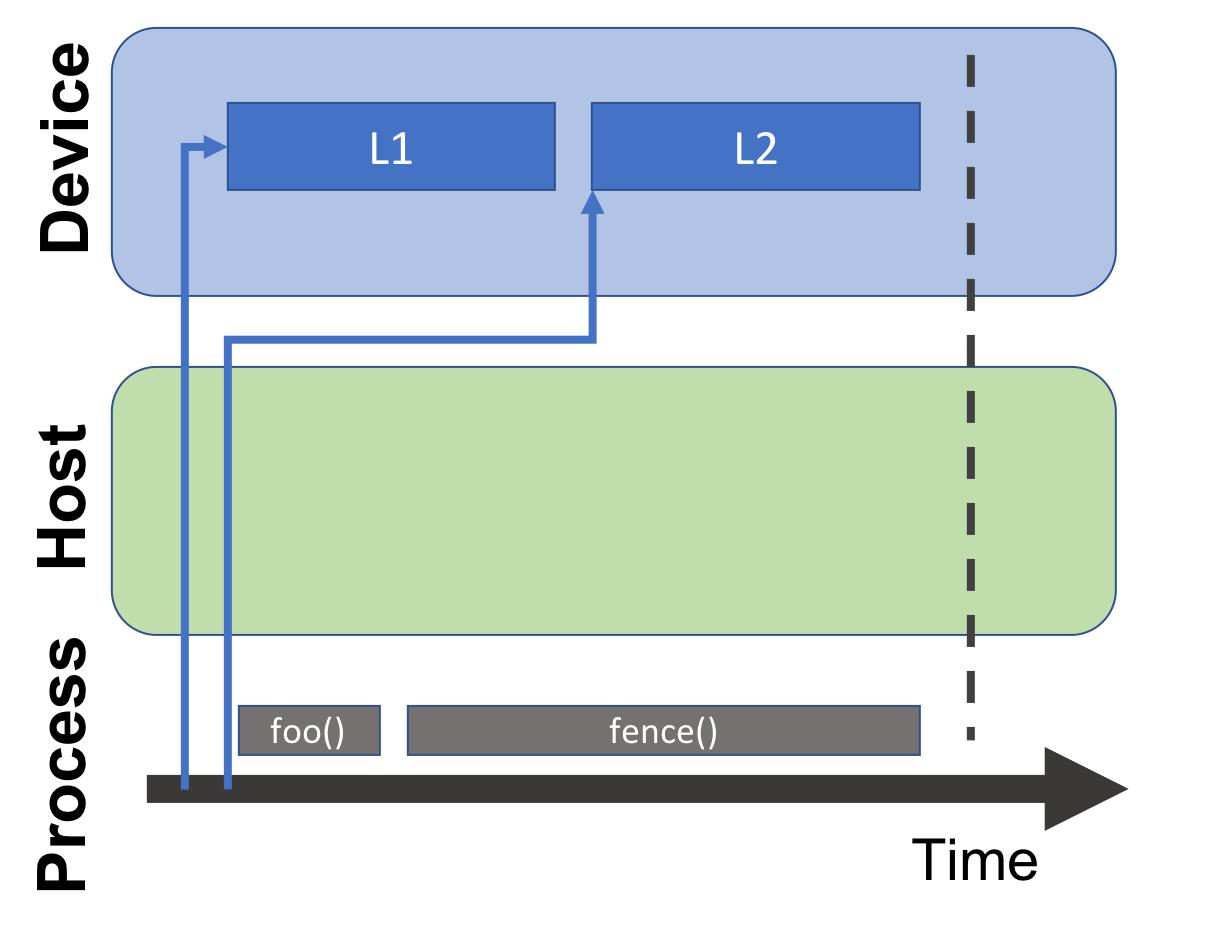
\includegraphics[width=0.95\textwidth]{figures/streams-fig1} 
 
    \end{column}

    \begin{column}{.33\textwidth}
	    \begin{code}[linebackgroundcolor={},keywords={L1,L2,policy_device}]
RangePolicy<> 
  policy_device(0,N)
FunctorL1 L1(...);
FunctorL2 L2(...);

parallel_for("L1", 
  policy_device, L1);
parallel_for("L2", 
  policy_device, L2);
foo();
fence();
      \end{code}
    \end{column}
  \end{columns}
\end{frame}

%==========================================================================

\begin{frame}[fragile]{Simple Dispatch}
  \textbf{Execution Spaces execute in dispatch order}
  \begin{itemize}
    \item{Dispatches to the same space instance will never overlap}
    \item{Executed in order FIFO}
    \item{Use \texttt{Kokkos::fence()} to wait for completion}
  \end{itemize}

  \begin{columns}[]
    \begin{column}{.67\textwidth}

       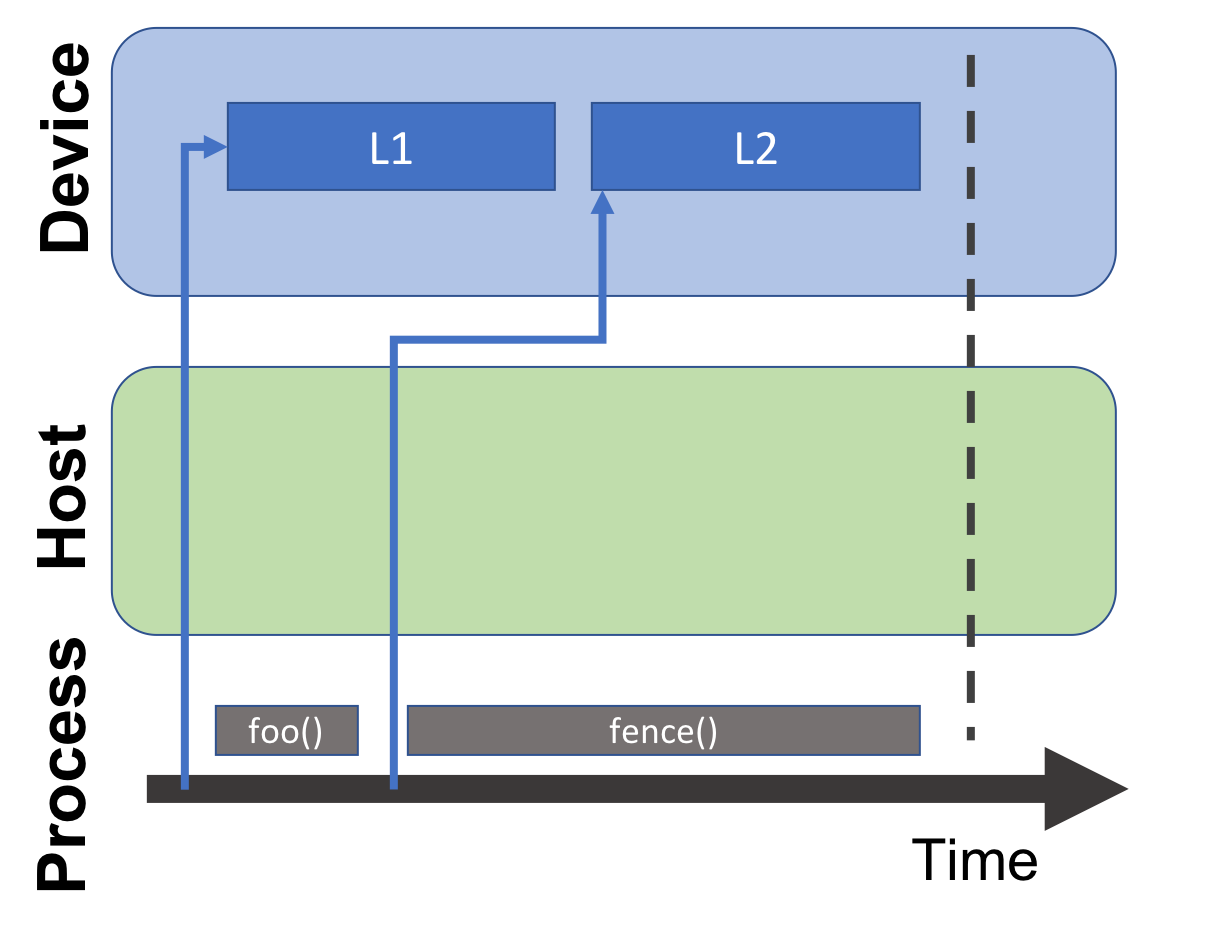
\includegraphics[width=0.95\textwidth]{figures/streams-fig2} 
 
    \end{column}

    \begin{column}{.33\textwidth}
	    \begin{code}[linebackgroundcolor={\btLstHL{8}{black!15}},keywords={L1,L2,policy_device}]
RangePolicy<> 
  policy_device(0,N)
FunctorL1 L1(...);
FunctorL2 L2(...);

parallel_for("L1", 
  policy_device, L1);
foo();
parallel_for("L2", 
  policy_device, L2);
fence();
      \end{code}
    \end{column}
  \end{columns}
\end{frame}

%==========================================================================

\begin{frame}[fragile]{Host/Device Dispatch}
  \textbf{ExecutionSpaces are Independent}
  \begin{itemize}
    \item{Dispatches into different ExecutionSpaces may overlap.}
    \item{Overlap with process thread functions and each other}
    \item{Use \texttt{Kokkos::fence()} to wait for completion of all}
  \end{itemize}

  \begin{columns}[]
    \begin{column}{.67\textwidth}

       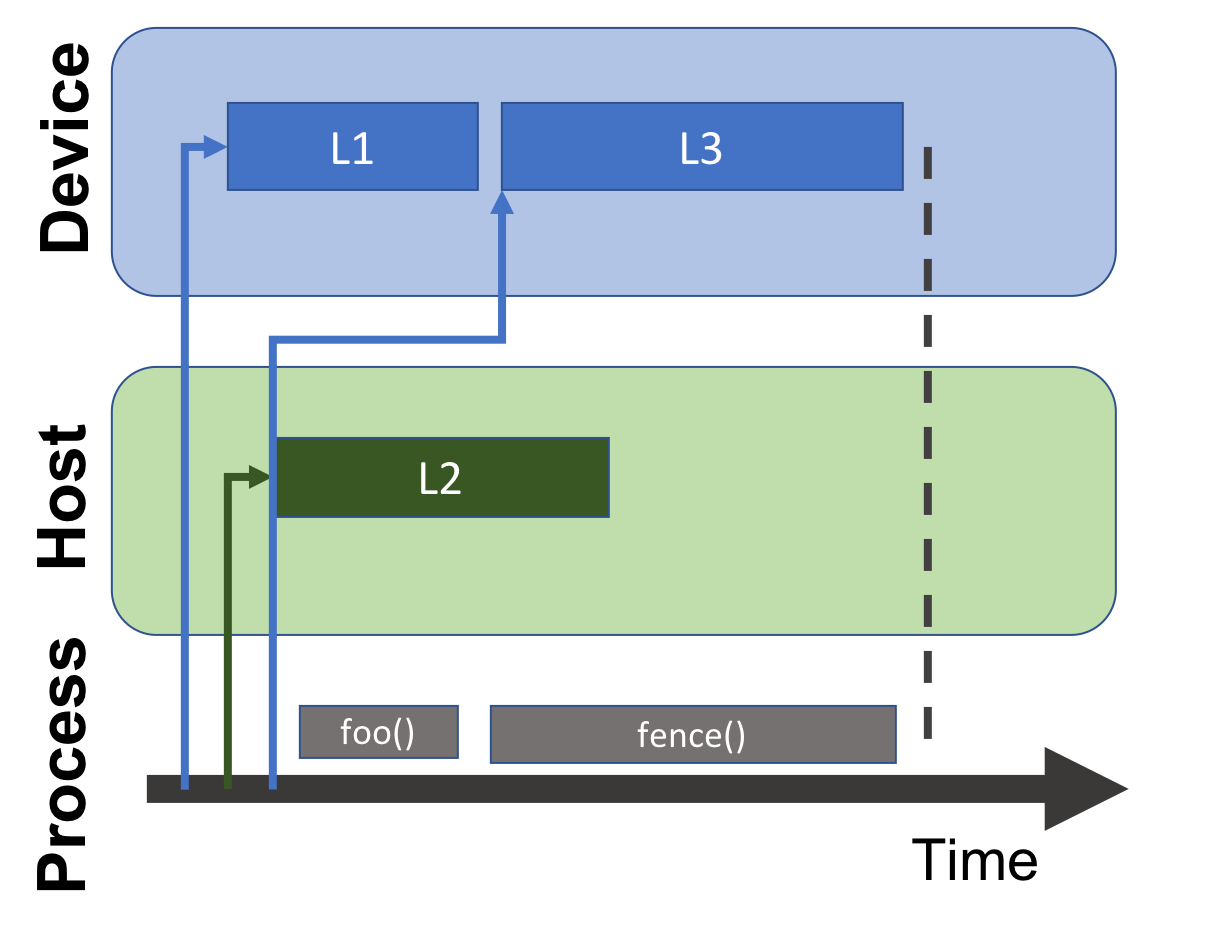
\includegraphics[width=0.95\textwidth]{figures/streams-fig3} 
 
    \end{column}

    \begin{column}{.33\textwidth}
	    \begin{code}[linebackgroundcolor={},keywords={L1,L2,L3,policy_device,policy_host}]
RangePolicy<> 
  policy_d(0,N)
RangePolicy<Host>
  policy_host(0,N)
FunctorL1 L1(...);
FunctorL2 L2(...);
FunctorL3 L3(...);
parallel_for("L1", 
  policy_d, L1);
parallel_for("L2", 
  policy_host, L2);
parallel_for("L3", 
  policy_d, L3);
foo();
fence();
      \end{code}
    \end{column}
  \end{columns}
\end{frame}

%==========================================================================

\begin{frame}[fragile]{Host/Device Dispatch Reality}
  \textbf{Reality: Some Host Backends Block}
  \begin{itemize}
  \item{Most host backends are blocking dispatches (except HPX)}
    \item{They never overlap with process thread functions}
    \item{But: \textbf{Do NOT rely on blocking behavior!!}}
  \end{itemize}

  \begin{columns}[]
    \begin{column}{.67\textwidth}

       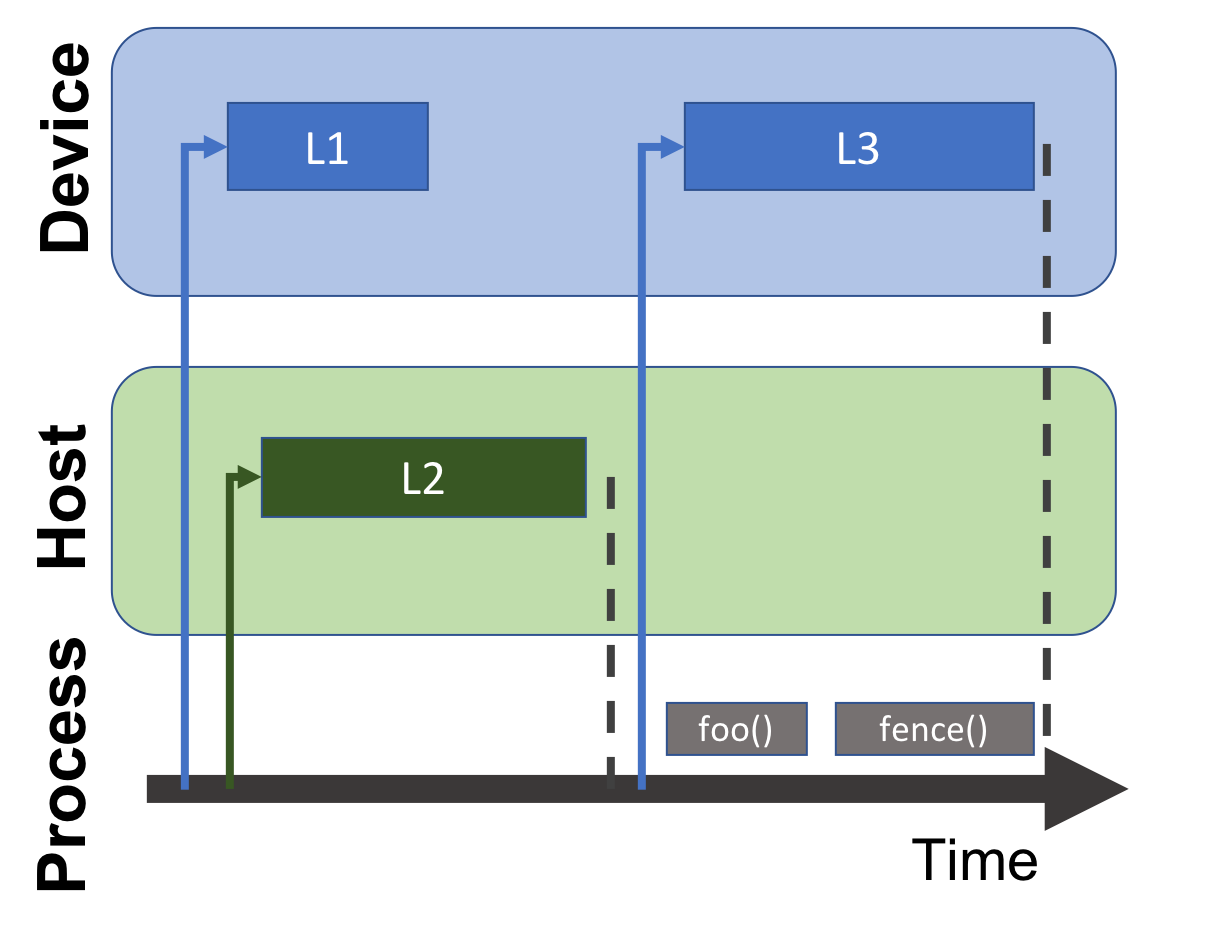
\includegraphics[width=0.95\textwidth]{figures/streams-fig4} 
 
    \end{column}

    \begin{column}{.33\textwidth}
	    \begin{code}[linebackgroundcolor={},keywords={L1,L2,L3,policy_device,policy_host}]
RangePolicy<> 
  policy_d(0,N)
RangePolicy<Host>
  policy_host(0,N)
FunctorL1 L1(...);
FunctorL2 L2(...);
FunctorL3 L3(...);
parallel_for("L1", 
  policy_d, L1);
parallel_for("L2", 
  policy_host, L2);
parallel_for("L3", 
  policy_d, L3);
foo();
fence();
      \end{code}
    \end{column}
  \end{columns}
\end{frame}

%==========================================================================

\begin{frame}[fragile]{Reductions}
  \textbf{Reductions to Scalars are Blocking}
  \begin{itemize}
    \item{The call only returns after result is available.}
    \item{FIFO implies, every other kernel in the same ExecutionSpace instance will be done too}
  \end{itemize}

  \begin{columns}[]
    \begin{column}{.67\textwidth}

       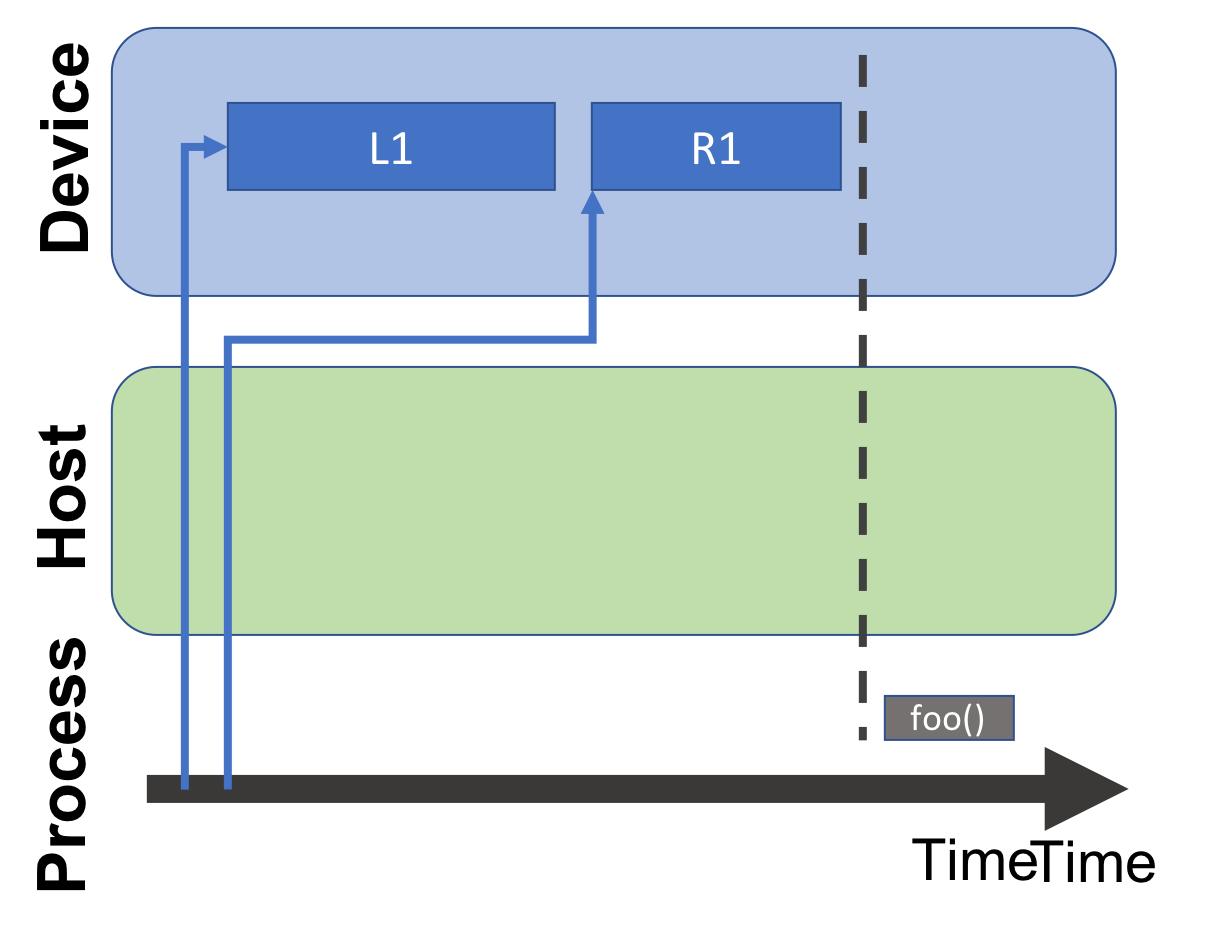
\includegraphics[width=0.95\textwidth]{figures/streams-fig5} 
 
    \end{column}

    \begin{column}{.33\textwidth}
	    \begin{code}[linebackgroundcolor={},keywords={L1,L2,policy_device}]
RangePolicy<> 
  policy_d(0,N)
FunctorL1 L1(...);
FunctorR1 R1(...);

double result;
parallel_for("L1", 
  policy_d, L1);
parallel_reduce("R1", 
  policy_d, R1, result);
foo();
      \end{code}
    \end{column}
  \end{columns}
\end{frame}

%==========================================================================

\begin{frame}[fragile]{Reductions to Scalars}
  \textbf{Reductions to Scalars are Blocking}
  \begin{itemize}
    \item{The call only returns after result is available.}
    \item{For subsequent dispatches previous rules apply}
  \end{itemize}

  \begin{columns}[]
    \begin{column}{.67\textwidth}

       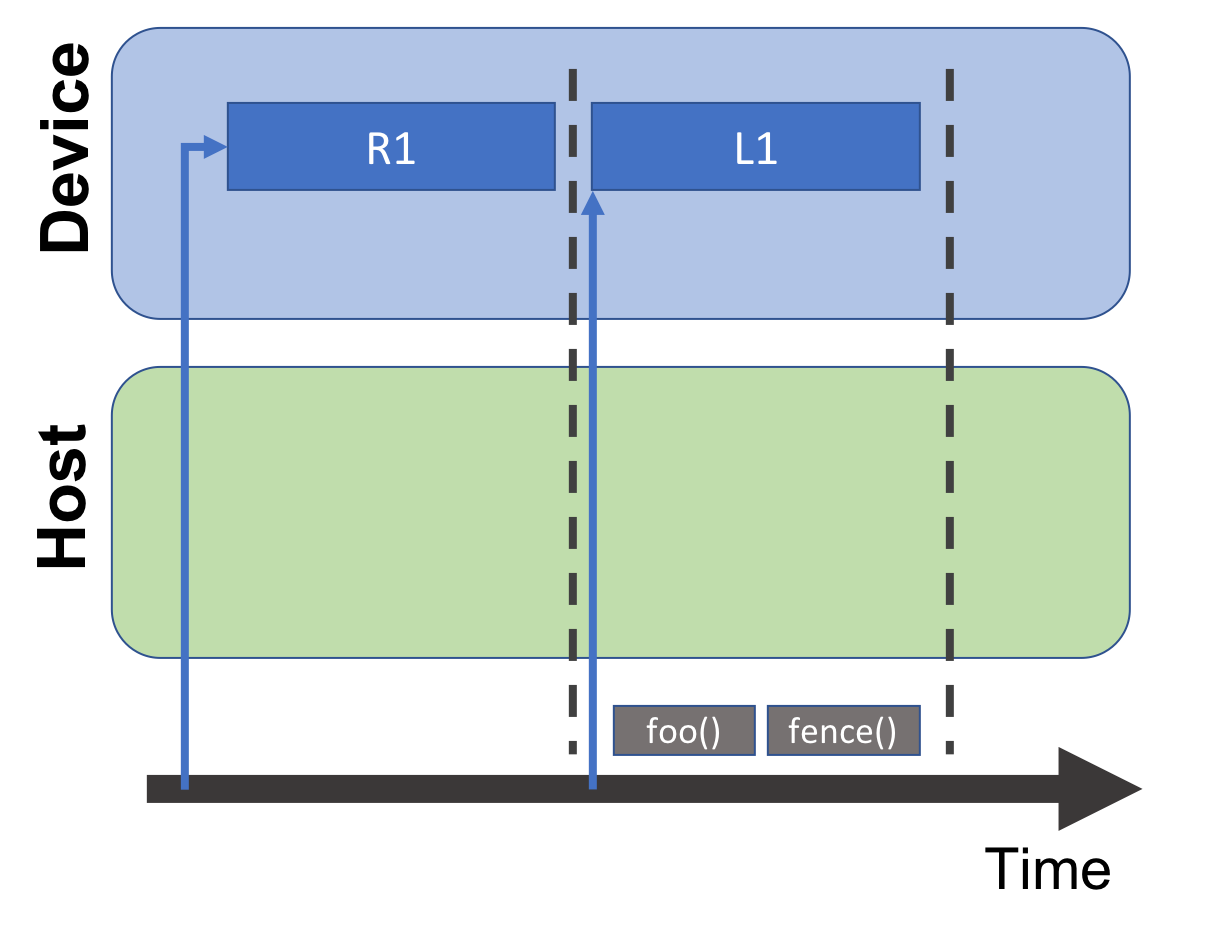
\includegraphics[width=0.95\textwidth]{figures/streams-fig6} 
 
    \end{column}

    \begin{column}{.33\textwidth}
	    \begin{code}[linebackgroundcolor={},keywords={L1,L2,policy_device}]
RangePolicy<> 
  policy_d(0,N)
FunctorL1 L1(...);
FunctorR1 R1(...);

double result;
parallel_reduce("R1", 
  policy_d, R1, result);
parallel_for("L1", 
  policy_d, L1);
foo();
fence();
      \end{code}
    \end{column}
  \end{columns}
\end{frame}

%==========================================================================

\begin{frame}[fragile]{Reductions to Views}
  \textbf{Reductions to Views are Non-blocking}
  \begin{itemize}
    \item{Behave like a \texttt{parallel\_for}}
    \item{Results are only available after a \texttt{Kokkos::fence()}}
    \item{Even true for unmanaged \texttt{View}s of host variables!}
  \end{itemize}

  \begin{columns}[]
    \begin{column}{.67\textwidth}

       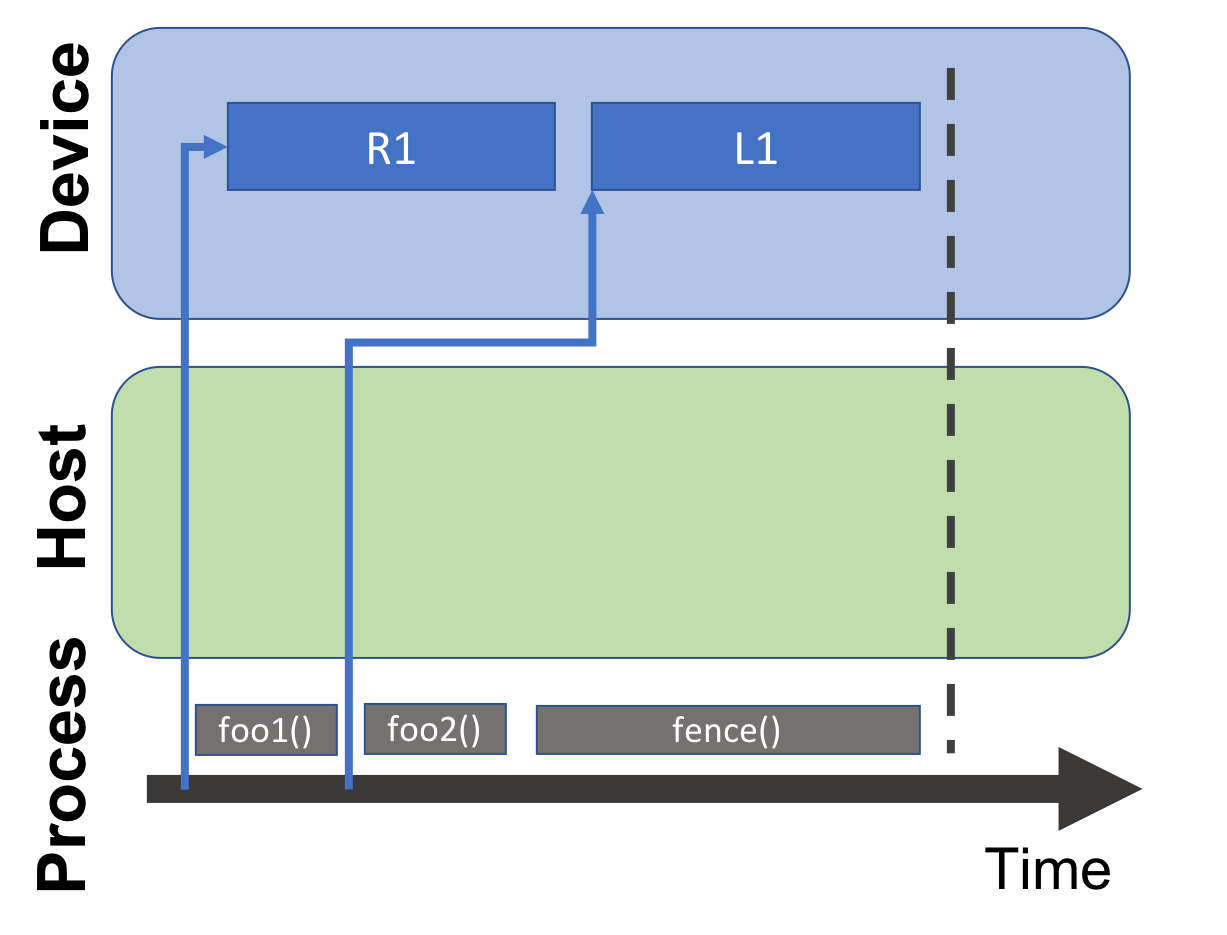
\includegraphics[width=0.95\textwidth]{figures/streams-fig7} 
 
    \end{column}

    \begin{column}{.33\textwidth}
    \begin{code}[linebackgroundcolor={},keywords={L1,L2,policy_device}]
...
double result;
View<double, HostSpace>
  v_result(&result);
parallel_reduce("R1", 
  policy_d,R1,v_result);
foo1();
parallel_for("L1", 
  policy_d, L1);
foo2();
fence();
      \end{code}
    \end{column}
  \end{columns}
\end{frame}

%==========================================================================

\begin{frame}[fragile]{Simple Dispatch}
  \textbf{Simple Parallel Loop}
  \begin{itemize}
    \item{Asynchronous}
    \item{Overlaps with host functions}
    \item{Use \texttt{Kokkos::fence()} to wait for completion}
  \end{itemize}

  \begin{columns}[]
    \begin{column}{.67\textwidth}

       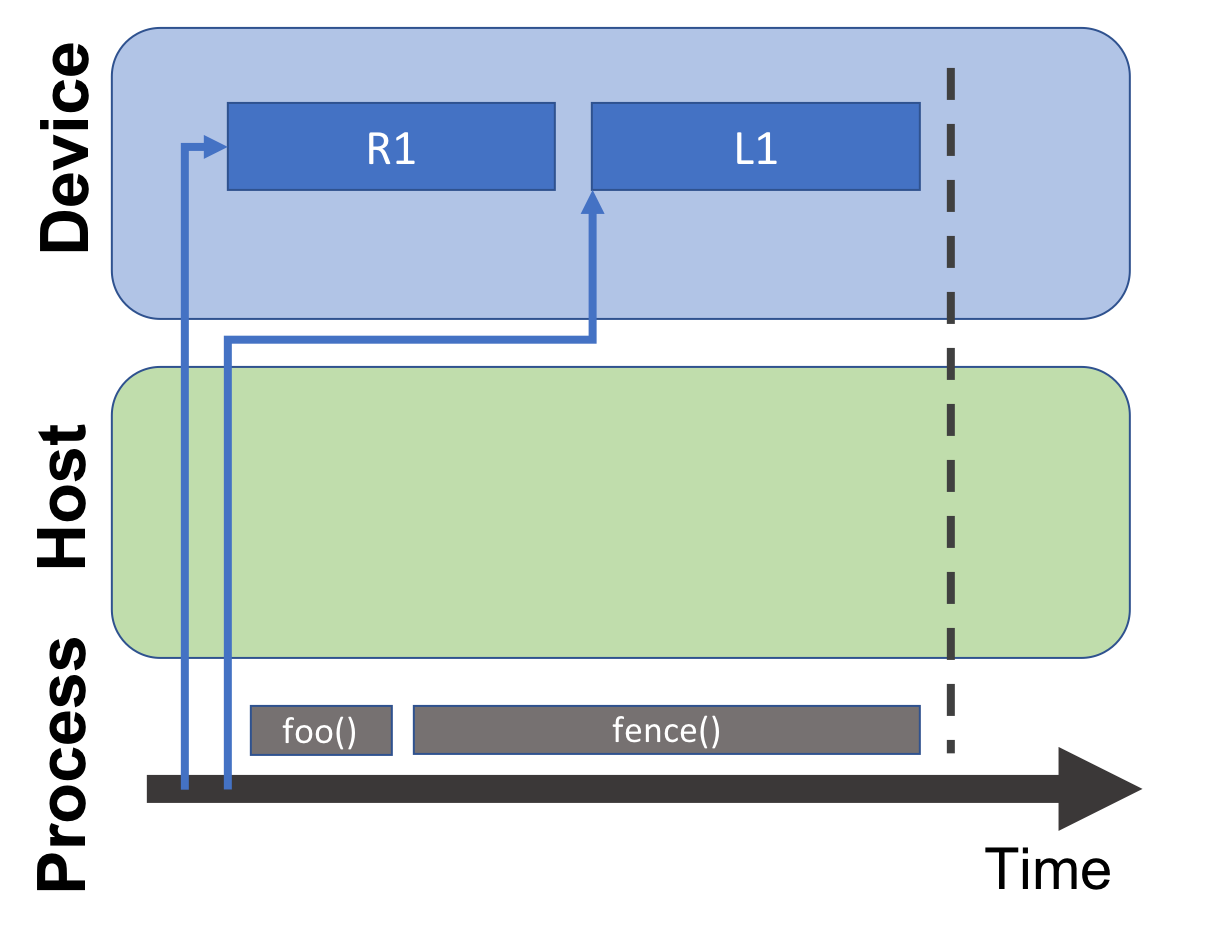
\includegraphics[width=0.95\textwidth]{figures/streams-fig8} 
 
    \end{column}

    \begin{column}{.33\textwidth}
	    \begin{code}[linebackgroundcolor={},keywords={L1,L2,policy_device}]
RangePolicy<> 
  policy_device(0,N)
FunctorL1 L1(...);
FunctorL2 L2(...);

parallel_for("L1", 
  policy_device, L1);
parallel_for("L2", 
  policy_device, L2);
foo();
fence();
      \end{code}
    \end{column}
  \end{columns}
\end{frame}

%==========================================================================

\begin{frame}[fragile]{Deep Copy}
  \textbf{2-Argument deep\_copy is fully blocking}
  \begin{itemize}
    \item{Implies a full \texttt{fence} before the copy}
    \item{Copy is done by the time call returns.}
    \item{Even if it is a no-op due to \texttt{src == dst}!}
  \end{itemize}

  \begin{columns}[]
    \begin{column}{.67\textwidth}

       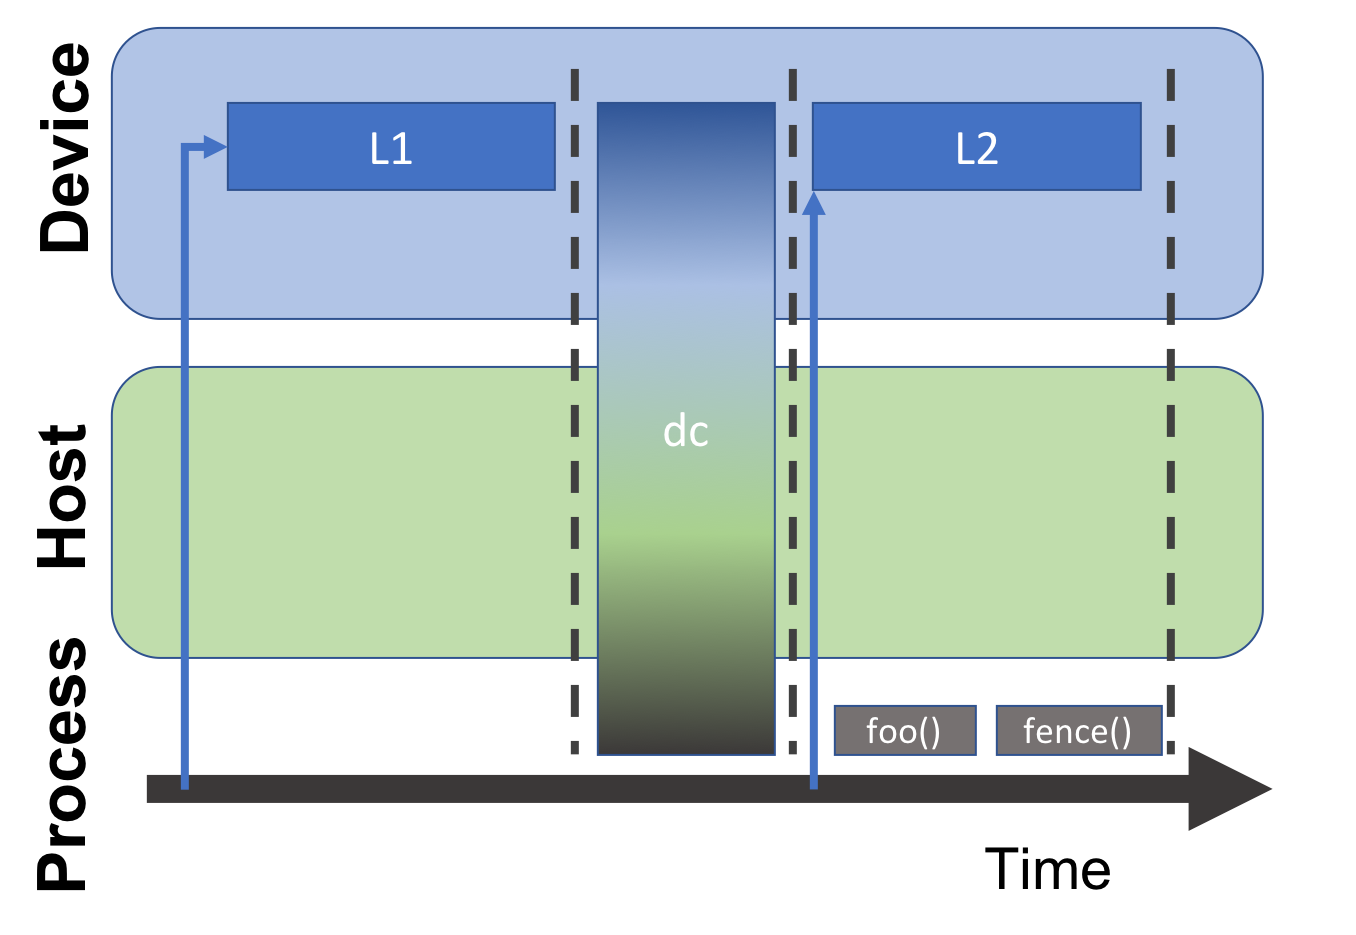
\includegraphics[width=0.95\textwidth]{figures/streams-fig9} 
 
    \end{column}

    \begin{column}{.33\textwidth}
	    \begin{code}[linebackgroundcolor={},keywords={L1,L2,policy_device}]

parallel_for("L1", 
  policy_device, L1);
deep_copy(dest,src);
parallel_for("L2", 
  policy_device, L2);
foo();
fence();
      \end{code}
    \end{column}
  \end{columns}
\end{frame}

%==========================================================================

\begin{frame}[fragile]{Deep Copy}
  \textbf{deep\_copy with space argument are non-blocking}
  \begin{itemize}
    \item{Execute in dispatch order in the queue of the space}
    \item{Overlap with host process functions}
    \item{Use \texttt{Kokkos::fence()} to wait for completion}
  \end{itemize}

  \begin{columns}[]
    \begin{column}{.67\textwidth}

       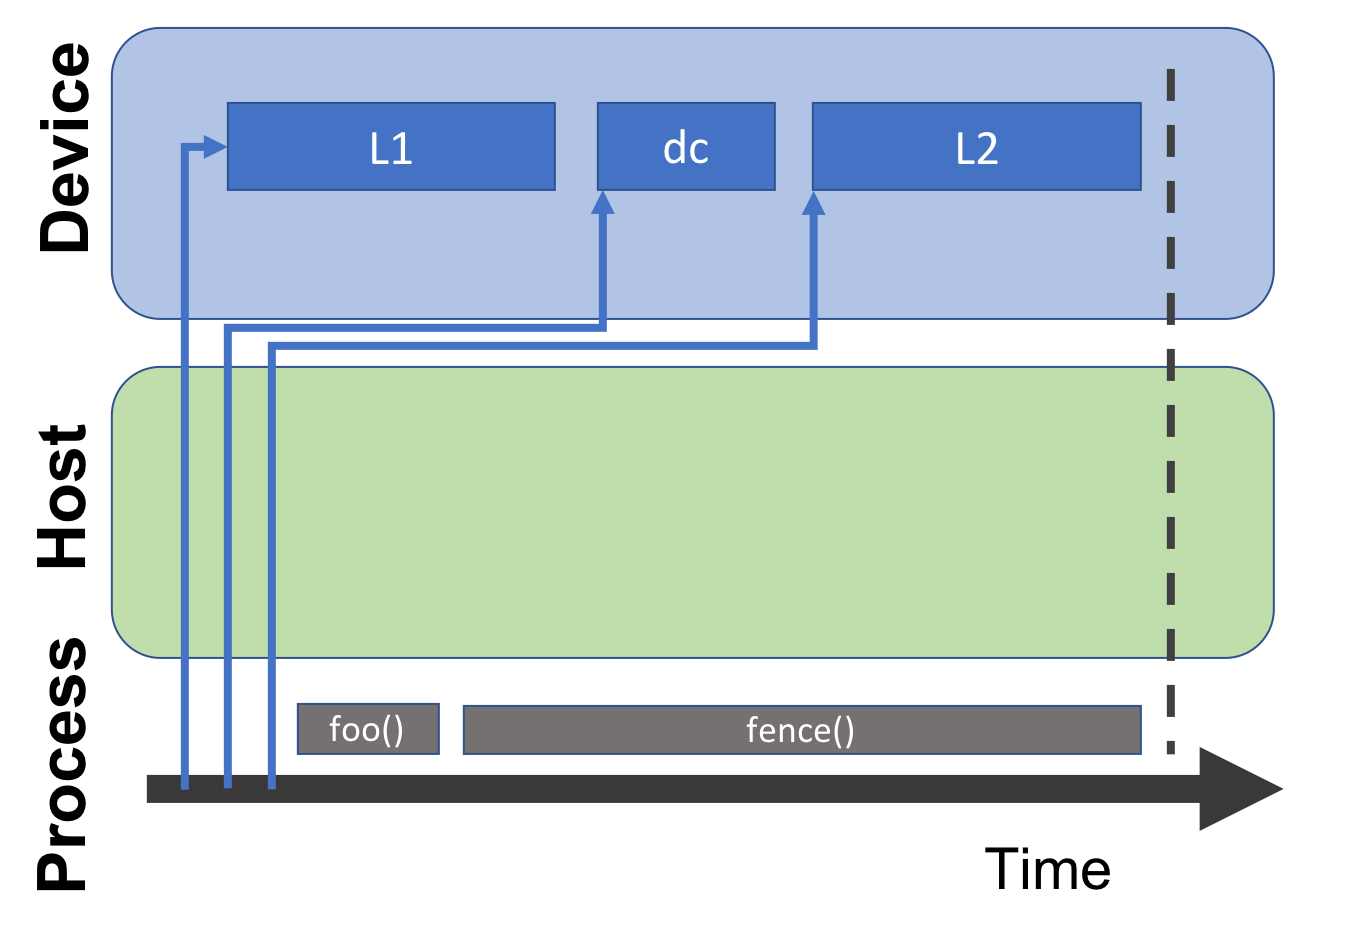
\includegraphics[width=0.95\textwidth]{figures/streams-fig10} 
 
    \end{column}

    \begin{column}{.33\textwidth}
	    \begin{code}[linebackgroundcolor={},keywords={L1,L2,policy_device}]
parallel_for("L1", 
  policy_device, L1);
deep_copy(device,
  dest,src);
parallel_for("L2", 
  policy_device, L2);
foo();
fence();
      \end{code}
    \end{column}
  \end{columns}
\end{frame}

%==========================================================================

\begin{frame}[fragile]{Deep Copy}
  \textbf{deep\_copy with space argument are non-blocking}
  \begin{itemize}
    \item{Execute in dispatch order in the queue of the space}
    \item{Overlap with other execution spaces}
    \item{Use \texttt{Kokkos::fence()} to wait for completion}
  \end{itemize}

  \begin{columns}[]
    \begin{column}{.67\textwidth}

       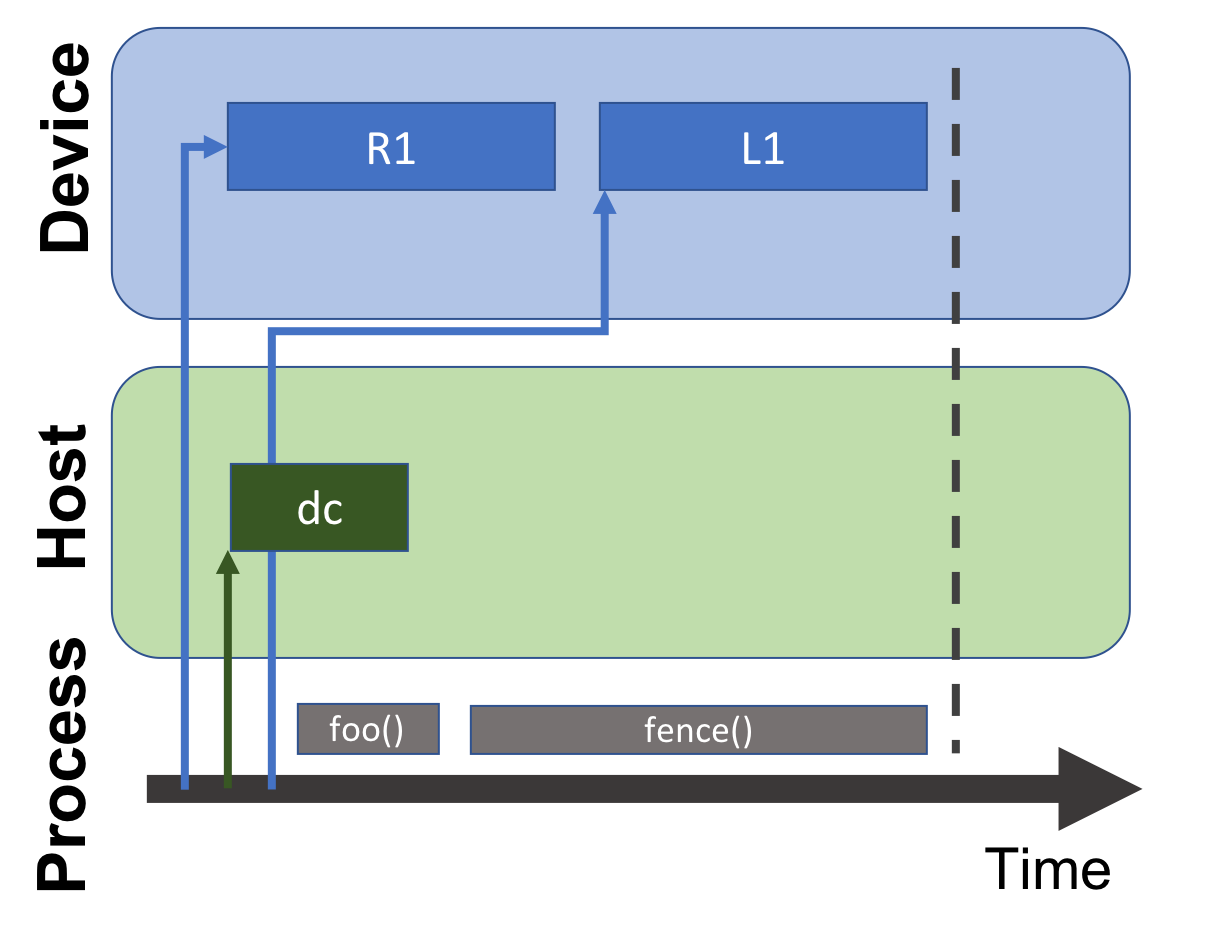
\includegraphics[width=0.95\textwidth]{figures/streams-fig11} 
 
    \end{column}

    \begin{column}{.33\textwidth}
	    \begin{code}[linebackgroundcolor={},keywords={L1,L2,policy_device}]
parallel_for("L1", 
  policy_device, L1);
deep_copy(host(),
  dest,src);
parallel_for("L2", 
  policy_device, L2);
foo();
fence();
      \end{code}
    \end{column}
  \end{columns}
\end{frame}

%==========================================================================

\begin{frame}[fragile]{Multiple Instances}
  \textbf{So what about CUDA streams?}

	Up to now we only used default execution space instances, but what if you want to have concurrent kernels on the GPU?

	\pause
	\begin{block}{Execution Space Instances}
		Execution Space instances behave largely like CUDA streams
	\end{block}

	\pause
	You can create different instances:
	\begin{itemize}
		\item Fairly new capability. 
		\item Initial version more for interoperability with CUDA/HIP.
		\begin{itemize}
			\item Give a \texttt{cudaStream\_t} to the constructor of the instance:
				\begin{code}[]
	cudaStream_t stream = ...;
	Kokkos::Cuda cuda_instance(stream);
				\end{code}
		\end{itemize}
		\item Generic versions upcoming (e.g. create generic instances)
		\item Not all spaces support having multiple distinct instances.
		\item ExecutionSpace instances are like shared pointers. 
	\end{itemize}

\end{frame}

%==========================================================================

\begin{frame}[fragile]{Multiple Instances}
  \textbf{Instances of Execution Spaces own a exec queue}
  \begin{itemize}
    \item{Work dispatched to different instances overlaps with each other}
    \item{Overlaps with host process functions}
    \item{Use \texttt{Kokkos::fence()} to wait for completion of all}
  \end{itemize}

  \begin{columns}[]
    \begin{column}{.67\textwidth}

       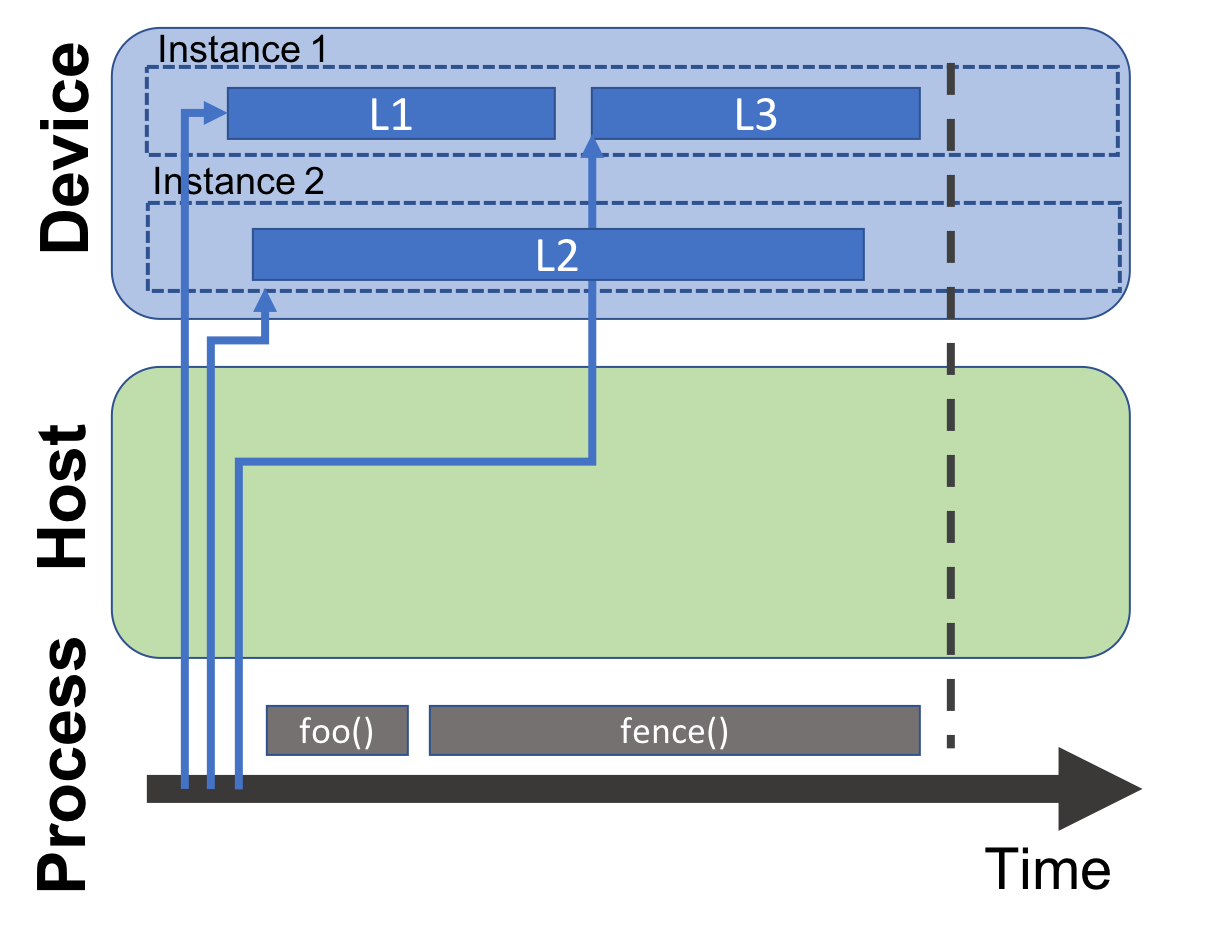
\includegraphics[width=0.95\textwidth]{figures/streams-fig12} 
 
    \end{column}

    \begin{column}{.33\textwidth}
	    \begin{code}[linebackgroundcolor={},keywords={L1,L2,policy_device}]
Device dev1(...);
Device dev2(...);
RangePolicy<Device>
  policy_d1(dev1,0,N);
RangePolicy<Device>
  policy_d2(dev2,0,N);

parallel_for("L1", 
  policy_d1, L1);
parallel_for("L2", 
  policy_d2, L2);
parallel_for("L3", 
  policy_d1, L3);
foo();
fence();
      \end{code}
    \end{column}
  \end{columns}
\end{frame}

%==========================================================================

\begin{frame}[fragile]{Multiple Instances}
  \textbf{deep\_copy with an instance argument also overlap}
  \begin{itemize}
    \item{deep\_copy with an instance argument are like any other parallel operation}
    \item{Overlaps with parallel operations in other instance}
  \end{itemize}

  \begin{columns}[]
    \begin{column}{.67\textwidth}

       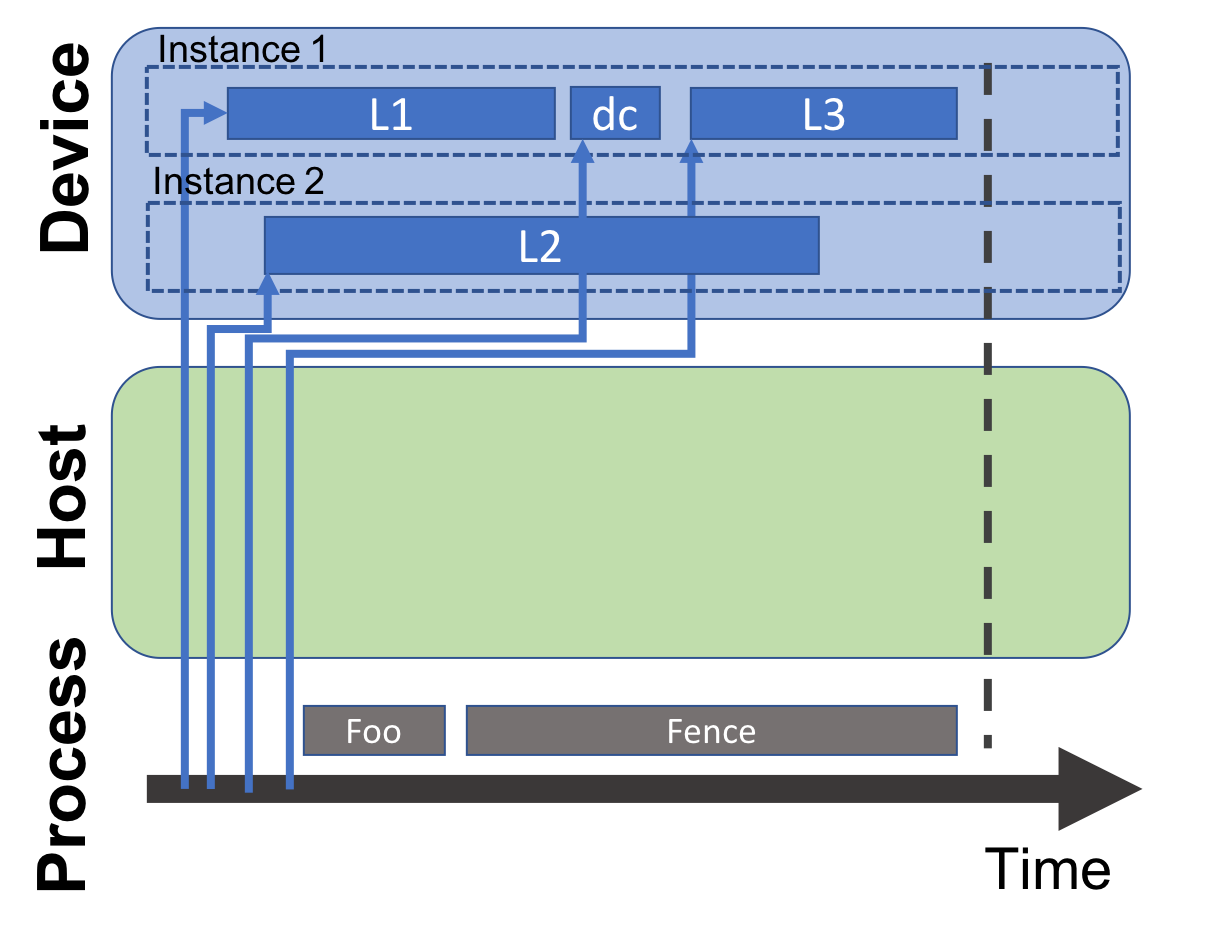
\includegraphics[width=0.95\textwidth]{figures/streams-fig13} 
 
    \end{column}

    \begin{column}{.33\textwidth}
	    \begin{code}[linebackgroundcolor={},keywords={L1,L2,policy_device}]
parallel_for("L1", 
  policy_d1, L1);
parallel_for("L2", 
  policy_d2, L2);
deep_copy(dev1,
  dest, src);
parallel_for("L3", 
  policy_d1, L3);
foo();
fence();
      \end{code}
    \end{column}
  \end{columns}
\end{frame}

%==========================================================================

\begin{frame}[fragile]{Fencing}
	\textbf{There are instance fences}
  \begin{itemize}
    \item{Use instance specific fence to only wait on that instance}
    \item{Operations in other instances can overlap with that fence}
    \item{Use \texttt{Kokkos::fence()} to wait for all outstanding ops}
  \end{itemize}

  \begin{columns}[]
    \begin{column}{.67\textwidth}

       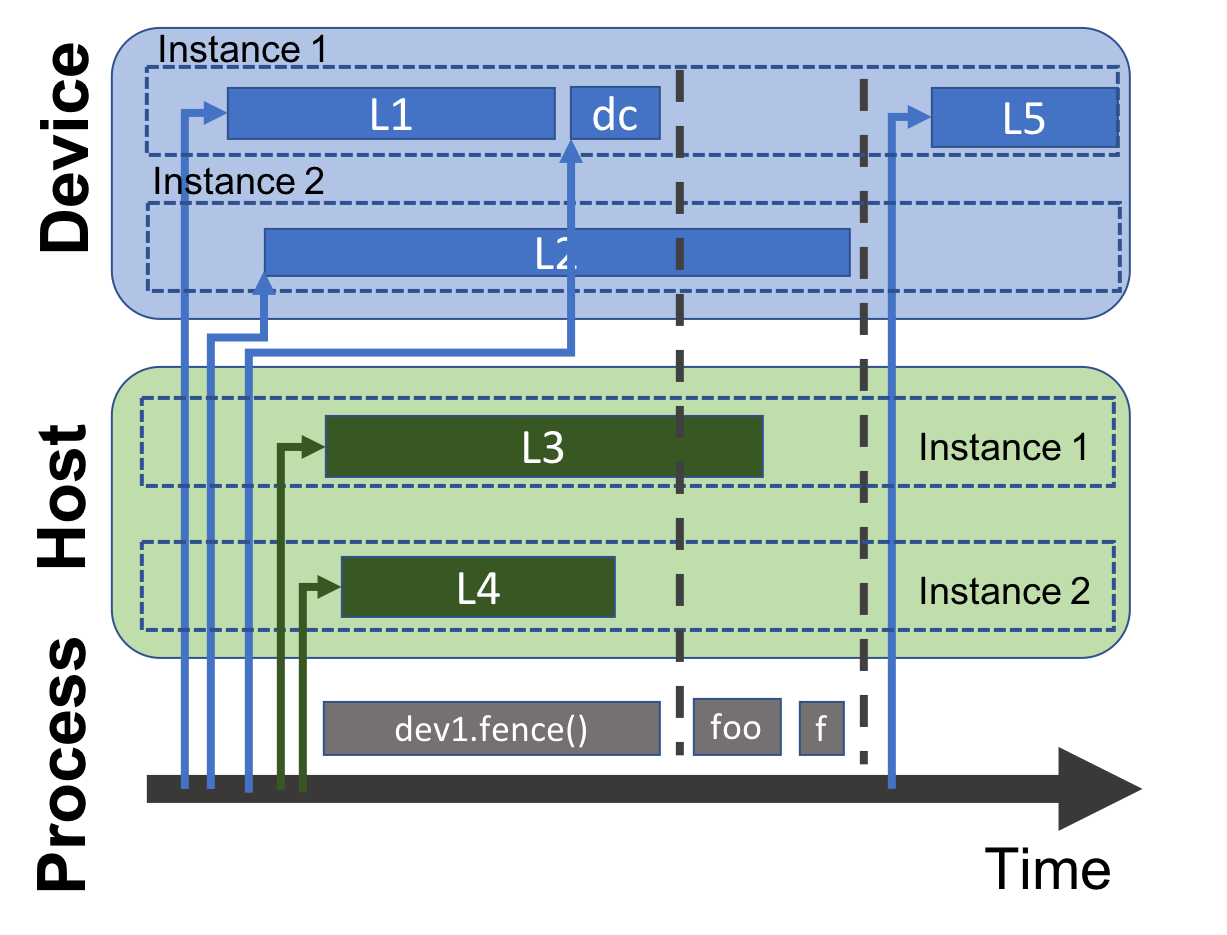
\includegraphics[width=0.95\textwidth]{figures/streams-fig14} 
 
    \end{column}

    \begin{column}{.33\textwidth}
	    \begin{code}[linebackgroundcolor={},keywords={L1,L2,policy_device}]
parallel_for("L1", 
  policy_d1, L1);
parallel_for("L2", 
  policy_d2, L2);
deep_copy(dev1,
  dest, src);
parallel_for("L3", 
  policy_h1, L3);
parallel_for("L4", 
  policy_h2, L4);
dev1.fence();
foo();
fence();
parallel_for("L5", 
  policy_d1, L5);
      \end{code}
    \end{column}
  \end{columns}
\end{frame}

%==========================================================================

\begin{frame}[fragile]{Deallocation}
	\textbf{Reality Check: Kokkos Views deallocation implies fence!}
  \begin{itemize}
    \item{Due to limitations of reference counting, deallocations fence!}
    \item{\textbf{Important:} this is implementation limitation not semantic!}
    \item{\textbf{Do NOT rely on deallocations fencing!}}
  \end{itemize}

  \begin{columns}[]
    \begin{column}{.67\textwidth}

       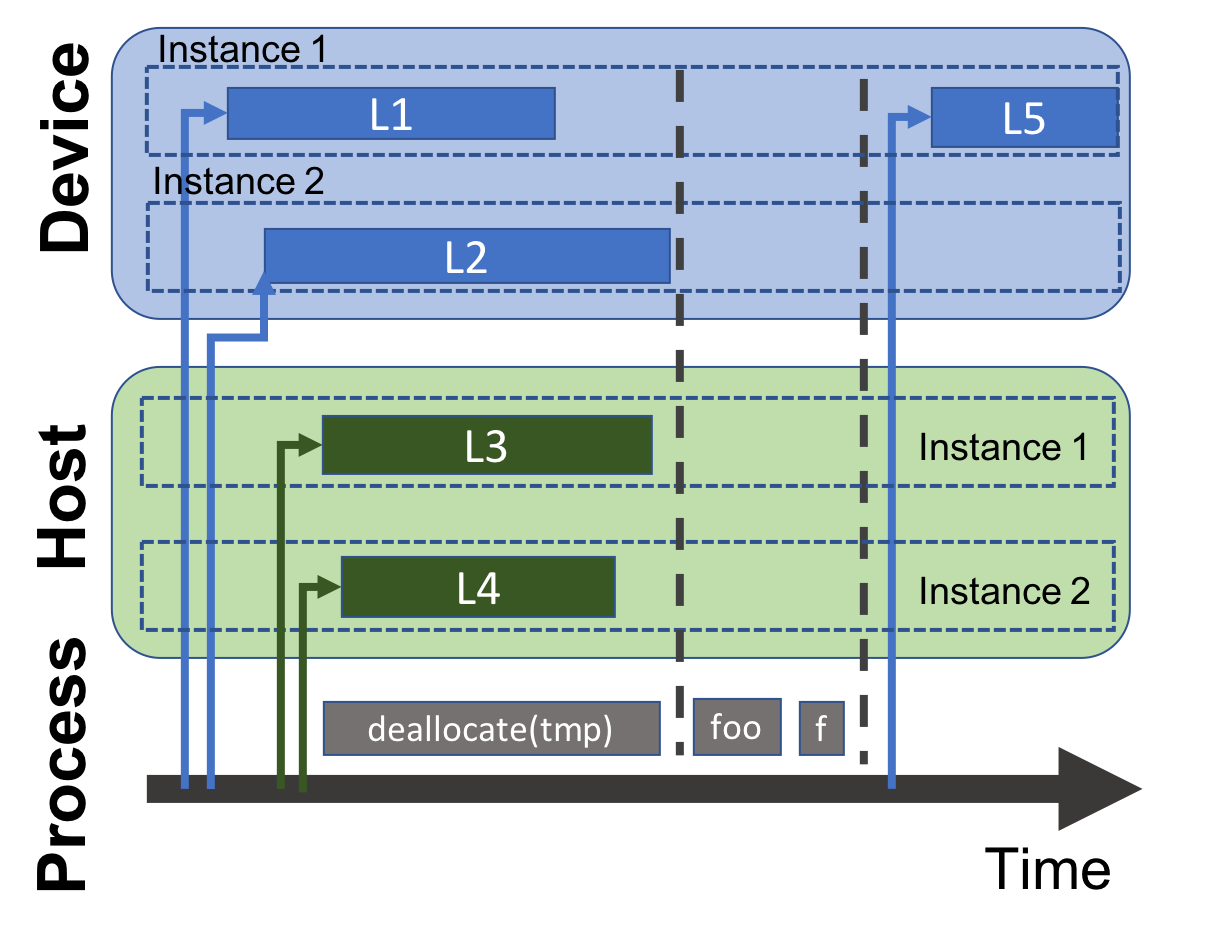
\includegraphics[width=0.95\textwidth]{figures/streams-fig15} 
 
    \end{column}

    \begin{column}{.33\textwidth}
	    \begin{code}[linebackgroundcolor={},keywords={L1,L2,policy_device}]
{
View<..> tmp(...);
parallel_for("L1", 
  policy_d1, L1);
parallel_for("L2", 
  policy_d2, L2);
parallel_for("L3", 
  policy_h1, L3);
parallel_for("L4", 
  policy_h2, L4);
}
foo();
fence();
parallel_for("L5", 
  policy_d1, L5);
      \end{code}
    \end{column}
  \end{columns}
\end{frame}


\begin{frame}{Section Summary}

  \begin{itemize}
    \item{Execution Space Instances execute work in order of dispatch.}
    \item{Operations dispatched to different Execution Space Instances can overlap.}
    \item{Each Execution Space type has a default instance as a singleton.}
    \item{Use \texttt{Kokkos::fence()} to wait for completion of ALL outstanding work.}
    \item{Use \texttt{exec\_space\_instance.fence()} to wait for completion of outstanding work dispatched to a specific execution space instance.}
  \end{itemize}

\end{frame}
